\myheader{Solution}{Assignment 8}{Internet Architecture}
\myquestion{MAC Addressing and ARP}

%----------------------------------------------------------------------------------------------
% Q1.a
%----------------------------------------------------------------------------------------------
\begin{enumerate}
    \item
        Consider the topology above and assign MAC addresses. For simplicity, it is 
        sufficient to provide the last 8 bits of the MAC address, i. e., two 
        characters in HEX notation (e. g., AB) as long as they are unique. You 
        do not have to assign MAC addresses to the “255 other hosts”.
\end{enumerate}
\begin{tcolorbox}
    \mysolution{} \\
    Figure \ref{fig:fig1} illustrates the topology given in the assignment
    with assigned MAC addresses and IP addresses. Only the last 8 bits of 
    the MAC address varies in different interfaces. 
\end{tcolorbox}

\begin{figure}[H]
    \begin{center}
        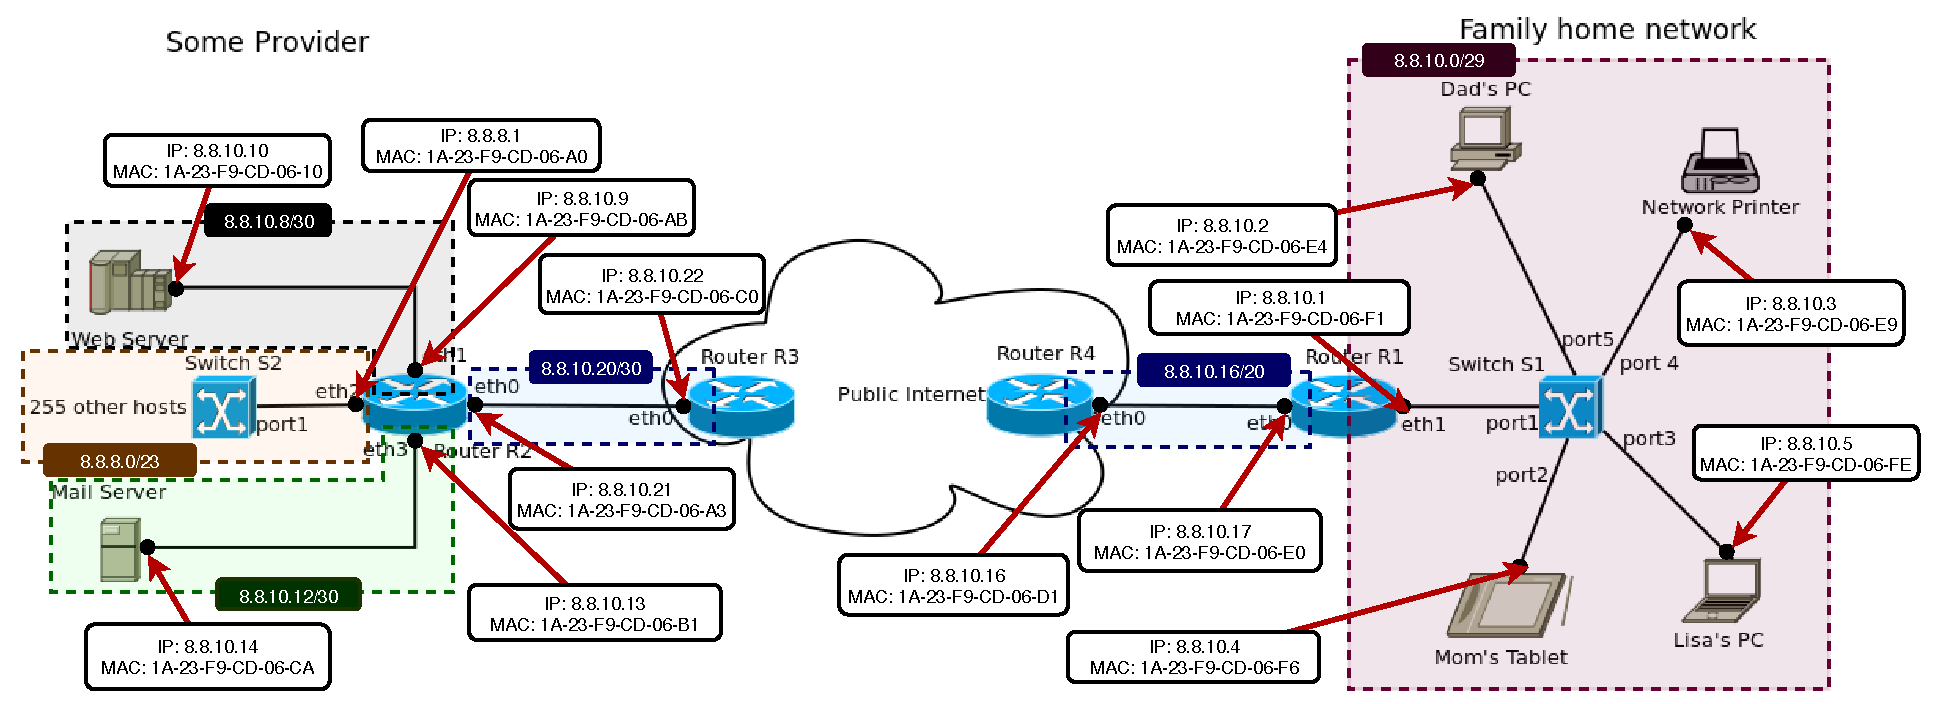
\includegraphics[scale=0.5]{HW08-Q01.pdf}
        \caption{Topology with assigned MAC addresses and IP addresses.}
        \label{fig:fig1}
    \end{center}
\end{figure}

%----------------------------------------------------------------------------------------------
% Q1.b
%----------------------------------------------------------------------------------------------
\begin{enumerate}
    \setcounter{enumi}{1}
    \item
    In the topology, clearly mark any broadcast and collision domain. How do these
    domains change when switch S2 is replaced by a hub?
\end{enumerate}

\begin{tcolorbox}
    \mysolution{} \\
    Figure \ref{fig:fig2} demonstrates the broadcast domains in the topology.
    The broadcast domains will not change if we change switch S2 to a hub. 

    Figure \ref{fig:fig3} illustrates the collision domains in the original 
    topology. Note that each host (from the 255 other hosts) will form a separate 
    collision domain. If switch S2 was replaced by a hub, then there would be 
    only one collision domain for all of them (See Figure \ref{fig:fig4}).
\end{tcolorbox}

\begin{figure}[H]
    \begin{center}
        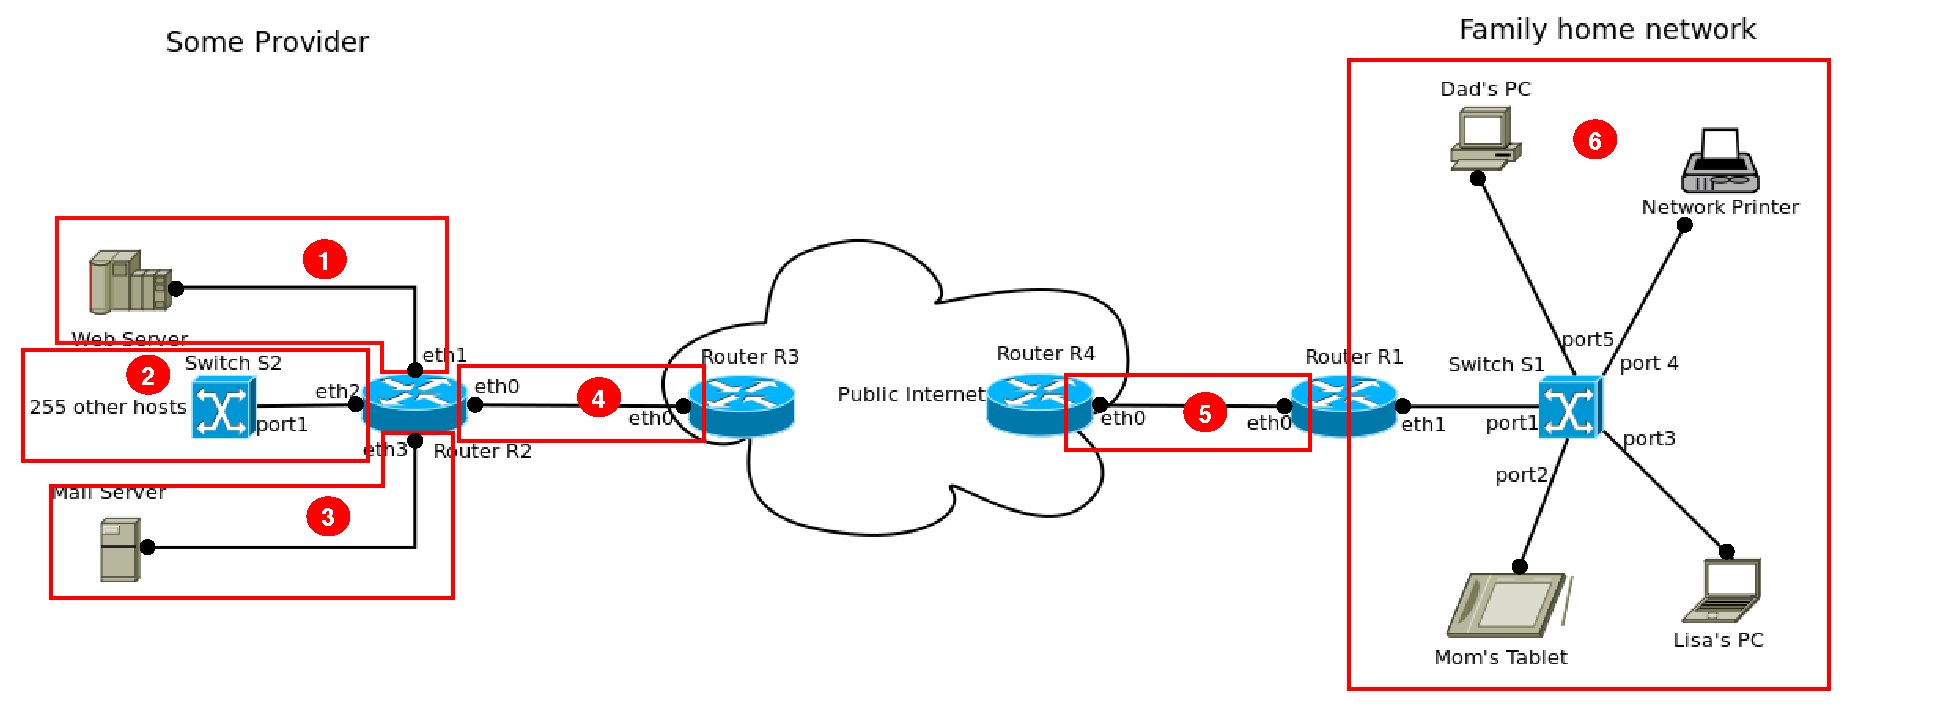
\includegraphics[scale=0.5]{fig2.pdf}
        \caption{Broadcast domains in both the original topology and in the topology
        where switch S2 is replaced by a hub.}
        \label{fig:fig2}
    \end{center}
\end{figure}

\begin{figure}[H]
    \begin{center}
        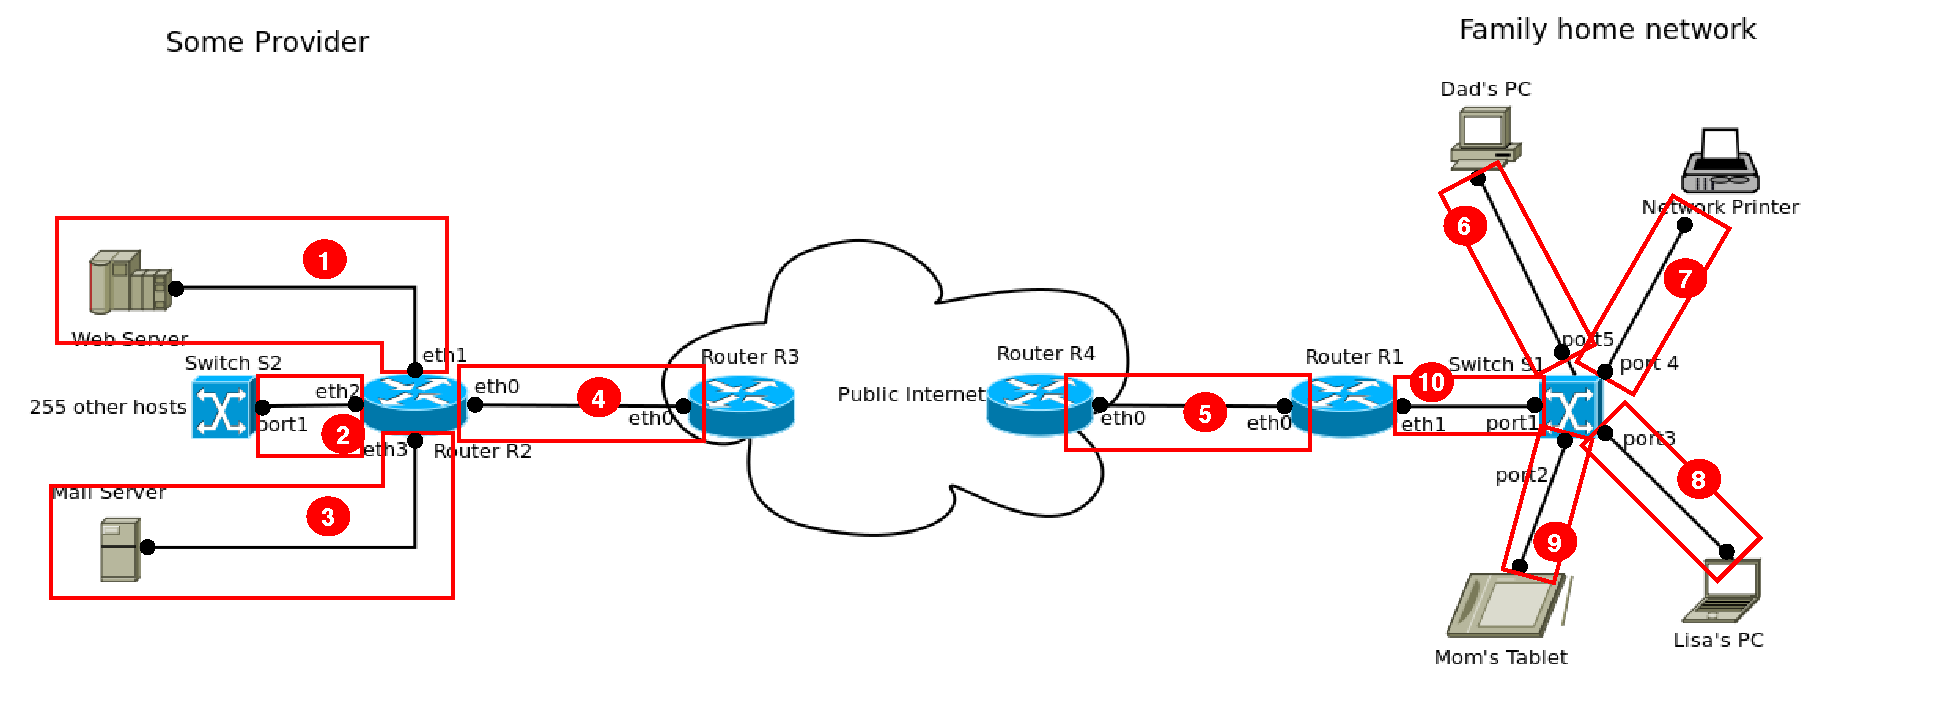
\includegraphics[scale=0.5]{fig3.pdf}
        \caption{Collision domains the original topology.}
        \label{fig:fig3}
    \end{center}
\end{figure}

\begin{figure}[H]
    \begin{center}
        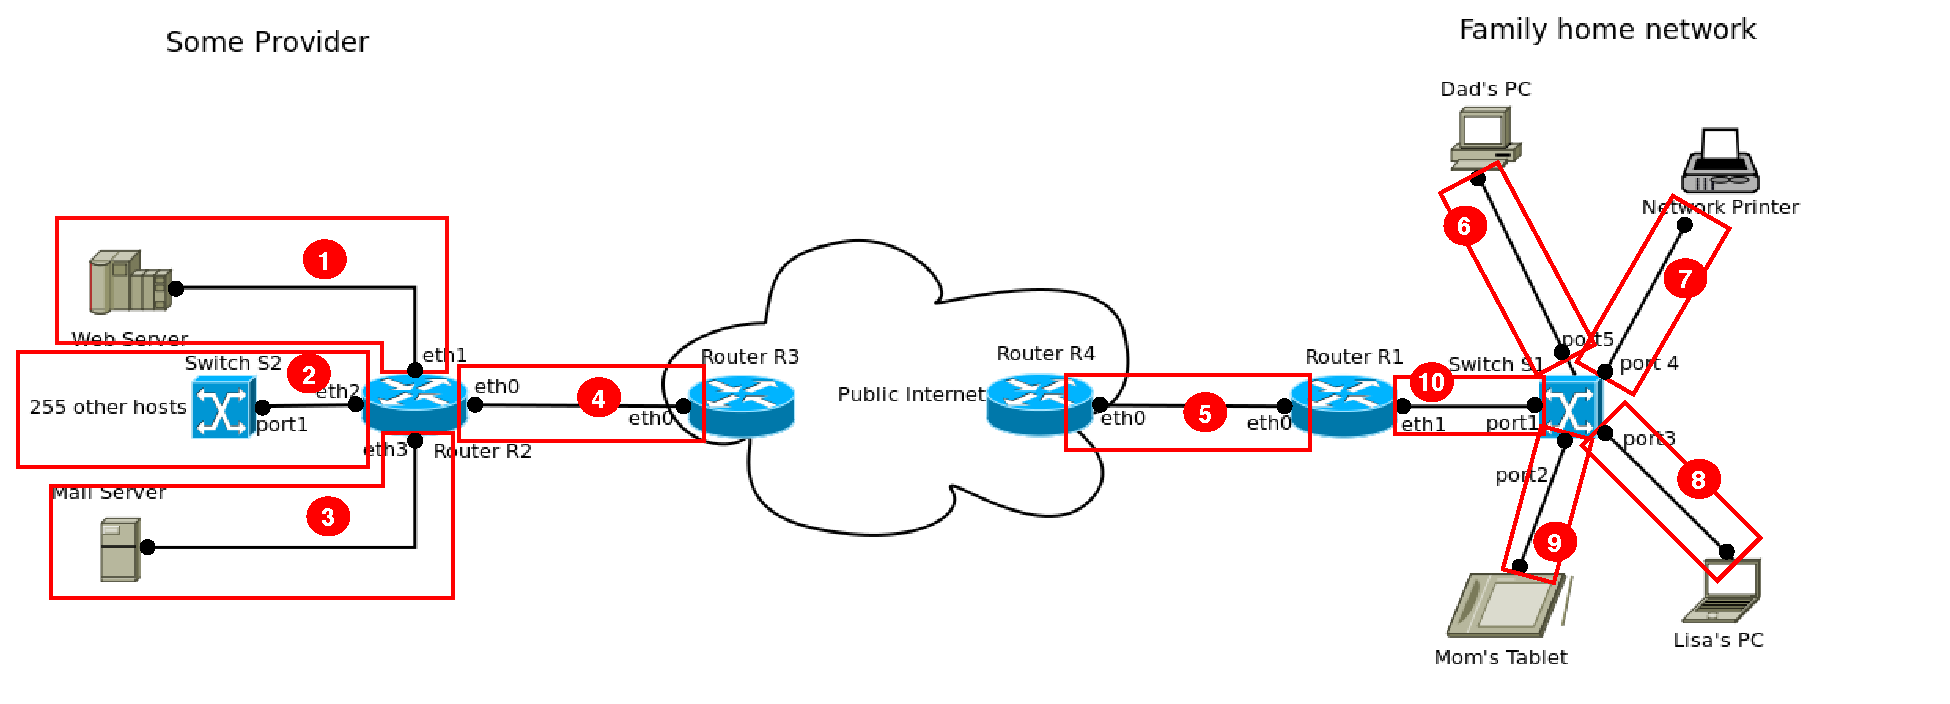
\includegraphics[scale=0.5]{fig4.pdf}
        \caption{Collision domains when switch S2 is replaced by a hub.}
        \label{fig:fig4}
    \end{center}
\end{figure}





%----------------------------------------------------------------------------------------------
% Q1.c
%----------------------------------------------------------------------------------------------
\begin{enumerate}
    \setcounter{enumi}{2}
    \item
        Which parts of the Ethernet, IP and TCP header will be modified when a packet is forwarded
        by i) router R1 / ii) switch S1?
\end{enumerate}

\begin{tcolorbox}
    \mysolution{} \\
    i) Router R1 changes Ethernet header and replace previous MAC addresses with new ones based
    on which path the packet should be forwarded to. Router also changes the TTL field from the 
    IP header.
    ii) Switch does not change any header field from the packet when it forwards a packet. 
\end{tcolorbox}


%----------------------------------------------------------------------------------------------
% Q1.c
%----------------------------------------------------------------------------------------------
\begin{enumerate}
    \setcounter{enumi}{3}
    \item
        Lisa wants to connect to the network printer via IP. Assume that all ARP caches 
        in the network are empty. What are the IP and MAC address fields of the ARP 
        messages exchanged to initiate the IP connection? Enter your results in a table 
        as in Tab. 1 for LAN segments E and F.
\end{enumerate}

\begin{tcolorbox}
    \mysolution{} \\
    Table \ref{tab:tab1} illustrates the messages exchanged to initiate the IP 
    connection between Lisa and network printer in which Lisa starts the connection.

\end{tcolorbox}

\begin{table}[H]
\label{tab:tab1}
    \caption{ARP messages exchanged to initiate the IP connection when Lisa wants to 
    connect to the network printer.}
\begin{tabular}{|c|c|c|c|c|c|}
\hline 
Index & LAN Segment    & Source IP & Source MAC        & Destination IP & Destination MAC   \\ \hline \hline
1     & E              & 8.8.10.5  & 1A-23-F9-CD-06-FE & 8.8.10.3       & FF-FF-FF-FF-FF-FF \\ \hline
2     & F, D, G, and H & 8.8.10.5  & 1A-23-F9-CD-06-FE & 8.8.10.3       & FF-FF-FF-FF-FF-FF \\ \hline
3     & F              & 8.8.10.3  & 1A-23-F9-CD-06-E9 & 8.8.10.5       & 1A-23-F9-CD-06-FE \\ \hline
4     & E              & 8.8.10.3  & 1A-23-F9-CD-06-E9 & 8.8.10.5       & 1A-23-F9-CD-06-FE \\ \hline
\end{tabular}
\end{table}


%----------------------------------------------------------------------------------------------
% Q1.d
%----------------------------------------------------------------------------------------------
\begin{enumerate}
    \setcounter{enumi}{4}
    \item
    What are the IP and MAC address fields of a response sent by the web server to Lisa’s 
    computer? Consider the response traversing all LAN segments drawn (A, B, C, D, E) and 
    enter your result in a table as in Tab. 1.
\end{enumerate}

\begin{tcolorbox}
    \mysolution{}  \\
    Table \ref{tab:tab2} shows the packets exchanged in the network to send a response 
    from the web server to Lisa's computer. We considered that all ARP cacehs in the 
    network are empty.

\end{tcolorbox}

\begin{table}[H]
\label{tab:tab2}
\caption{Packets exchanged in the topology to send a response from the web server
    to Lisa's computer, considering all ARP caches in the network are empty.}
\begin{tabular}{|c|c|c|c|c|c|c|}
\hline
Index & LAN Segment    & Source IP & Source MAC        & Destination IP & Destination MAC   \\ \hline
1     & A              & 8.8.10.10 & 1A-23-F9-CD-06-10 & 8.8.10.9       & FF-FF-FF-FF-FF-FF \\ \hline
2     & A              & 8.8.10.9  & 1A-23-F9-CD-06-AB & 8.8.10.10      & 1A-23-F9-CD-06-10 \\ \hline
3     & A              & 8.8.10.10 & 1A-23-F9-CD-06-10 & 8.8.10.5       & 1A-23-F9-CD-06-AB \\ \hline
4     & B              & 8.8.10.21 & 1A-23-F9-CD-06-A3 & 8.8.10.22      & FF-FF-FF-FF-FF-FF \\ \hline
5     & B              & 8.8.10.22 & 1A-23-F9-CD-06-C0 & 8.8.10.21      & 1A-23-F9-CD-06-A3 \\ \hline
6     & B              & 8.8.10.10 & 1A-23-F9-CD-06-A3 & 8.8.10.5       & 1A-23-F9-CD-06-C0 \\ \hline
7     & C              & 8.8.10.16 & 1A-23-F9-CD-06-D1 & 8.8.10.17      & FF-FF-FF-FF-FF-FF \\ \hline
8     & C              & 8.8.10.17 & 1A-23-F9-CD-06-E0 & 8.8.10.16      & 1A-23-F9-CD-06-D1 \\ \hline
9     & C              & 8.8.10.10 & 1A-23-F9-CD-06-D1 & 8.8.10.5       & 1A-23-F9-CD-06-E0 \\ \hline
10    & D              & 8.8.10.1  & 1A-23-F9-CD-06-D1 & 8.8.10.5       & FF-FF-FF-FF-FF-FF \\ \hline
11    & E, F, G, and H & 8.8.10.1  & 1A-23-F9-CD-06-D1 & 8.8.10.5       & FF-FF-FF-FF-FF-FF \\ \hline
12    & E              & 8.8.10.5  & 1A-23-F9-CD-06-FE & 8.8.10.1       & 1A-23-F9-CD-06-D1 \\ \hline
13    & D              & 8.8.10.5  & 1A-23-F9-CD-06-FE & 8.8.10.1       & 1A-23-F9-CD-06-D1 \\ \hline
14    & D              & 8.8.10.10 & 1A-23-F9-CD-06-D1 & 8.8.10.5       & 1A-23-F9-CD-06-FE \\ \hline
15    & E              & 8.8.10.10 & 1A-23-F9-CD-06-D1 & 8.8.10.5       & 1A-23-F9-CD-06-FE \\ \hline
\end{tabular}
\end{table}
